%!TEX encoding = UTF-8 Unicode
\chapter{静态分析}
静态分析是指不将样本中的代码实际运行起来的逆向分析。它的优点包括:
\begin{itemize}
  \item 理论上可以得到样本的全部代码和行为
  \item 不需要真实的运行环境
  \item 分析速度较快
  \item 适合自动化分析
  \item 是检测技术的主要基础
\end{itemize}

但静态分析也不是万能的。当样本的代码比较复杂时,静态分析需要很长的时间,而相比起来动态监控也许能得到更直观的结果。此外,如果样本有使用代码混淆,静态分析将极难进行。

对Android样本的静态分析包括:
\begin{itemize}
  \item 对Android XML格式的解码
  \item 对DEX文件格式的解析
  \item 对Dalvik指令的“反汇编”(即等价转换为适合于人阅读的形式)
  \item 对Dalvik指令的反编译
  \item 对ELF文件格式的解析
  \item 对ARM指令的反汇编
  \item 对ARM指令的反编译
\end{itemize}

其中,对ARM的静态分析将在第\ref{Chap:arm}章单独介绍。

\section{AXML解码}
\label{Sec:xml-decode}
Android中大量使用XML,用于项目配置(AndroidManifest.xml)、界面布局、字符串资源等。其中,AndroidManifest.xml中描述了应用程序的基本组件及其参数,这些基本组件可以说是恶意代码分析的“入口点”;此外,其中还包括应用程序运行所申请的额外的安全权限,这也是Android系统安全机制的一个重要组成部分。

但在APK文件中,这些XML文件并不是直接被压缩进去的,而是先被转成了一种特殊的格式(通常称之为AXML格式\index{AXML}),然后再被打包压缩到APK文件。在Android系统中,这些AXML格式文件也不会被还原为XML明文,而是直接进行解析。可惜的是,这种格式的文件,其内容无法直接被阅读。

为什么需要这么做?传统的XML解析有两种模型:SAX(Simple API for XML)和DOM(Document Object Model)。SAX的主要思路是遍历整个XML文件,每次遇到不同的对象(例如一个属性、一个节点开始、一个节点结束等),就触发相应的回调函数对其进行处理。这种解析方法的内存占用很少,适合于只需要遍历XML文件一次或少数几次就能把需要的事情都处理完的应用场景。但在Android中,由于AndroidManifest.xml会被多次使用(比如说,每次调用敏感API时都要检查其权限),所以并不适合使用SAX。DOM的主要思想则是将XML视为一棵树,在内存中建立并长期维护这颗树,而所有对XML的解析都变成对这颗树的访问。它的优点是可以每次访问都很快,甚至可以并行地方法(存在一定的读写互斥问题,这是另一个很有意思的话题)。但它的缺点也很明显,即需要长期占用较大的内存,对手机设备来说,内存是很重要的资源,这种消耗是应该要避免的。

实际上还有一种解析模型,叫PULL\footnote{\url{http://www.xmlpull.org}},它是SAX和DOM的折中方案。它很类似于SAX的事件触发机制,但这种触发并不调用事先注册的回调函数,而是由解析者自己触发事件并根据实际情况做自己的事情。由于这种主动性,即解析者可以自己决定哪些地方是感兴趣的、哪些地方不是,所以可以非常轻量地跳转到自己需要的那一部分数据做解析。

已经说得比较远了。之所以介绍PULL,是因为Android不但使用了PULL,还为PULL模型专门设计了AXML格式,这种格式的PULL解析非常容易实现,解析速度很快。此外,AXML还将所有字符串使用UTF-16LE编码、所有字段4字节内存对齐(Dalvik虚拟机和ARM处理器在访问4字节对齐数据时都会更快)、对重复字符串资源做成单实例等优化、根据需要解析字符串等。通过这些优化,进一步提高了Android系统解析XML文件的效率。

\subsection{AXMLPrinter2}
\lstinline!AXMLPrinter!\index{AXMLPrinter}是开源项目android4me\footnote{\url{http://code.google.com/p/android4me/}}的一个产品,可以将从XML到AXML的编码过程逆向执行,即将AXML文件还原为可读的XML形式。它的使用非常简单:
\begin{lstlisting}[language=bash, numbers=none]
 $ java -jar AXMLPrinter2.jar encoded.xml > decoded.xml
\end{lstlisting}

\subsection{其他}
如果要在自己的工具中实现AXML解码,通过外部命令行调用AXMLPrinter也许不方便,这时候需要可复用的源码。下面是推荐的源码:

\begin{table}[htbp]
  \caption{AXML解析源码}
  \centering
  \begin{tabular}{lll}
    \toprule
    项目 & 语言 & 地址 \\
    \midrule
    AXMLPrinter & Java & \url{http://code.google.com/p/android4me/} \\
    androguard & Python &  \url{http://code.google.com/p/androguard/}\\
    AndTools & C & \url{https://www.github.com/claudxiao/AndTools} \\
    \bottomrule
  \end{tabular}
\end{table}

\section{Dalvik反汇编}
APK文件中的classes.dex文件用于在Dalvik虚拟机中被加载和执行,对它的逆向是静态分析的主要工作。本节介绍将其opcode反汇编为可阅读指令的工具,但该文件的格式、这些指令的含义,均在后面第\ref{Chap:dalvik}章专门介绍。

\subsection{smali}
\lstinline!smali!\footnote{\url{http://code.google.com/p/smali/}}\index{smali}工具由两个文件smali.jar!和baksmali.jar组成。

baksmali.jar用于反汇编:
\begin{lstlisting}[language=bash, numbers=none]
 $ java -jar baksmali.jar classes.dex -o dir
\end{lstlisting}
上述命令会在dir目录下输出classes.dex的反汇编结果,每个Java类一个文件,扩展名为.smali,并以Java包名来组织路径。例如,\lstinline!com.example.Hello!类将生成com/example/Hello.smali文件。

smali.jar则用于将.smali文件汇编为DEX文件:
\begin{lstlisting}[language=bash, numbers=none]
 $ java -jar baksmali.jar dir -o classes_new.dex
\end{lstlisting}

\lstinline!smali!使用基于\lstinline!jasmin!\footnote{\url{http://jasmin.sourceforge.net}}\index{jasmin}的汇编语法。lohan+为这种语法编写了UltraEdit、Notepad++、Vim和SyntaxHighlighter的语法高亮文件,可以在其博客上下载\footnote{\url{http://androicracking.blogspot.com}}。这个博客还提供了一些逆向分析教程和资料。

因为精确地汇编与反汇编,\lstinline!smali!成为Android恶意代码编写和分析中最常用的工具之一。

\subsection{dedexer}
\lstinline!dedexer!\footnote{\url{http://sourceforge.net/projects/dedexer/}}\index{dedexer}是另一个Dalvik反汇编工具,用法是:
\begin{lstlisting}[language=bash, numbers=none]
 $ java -jar ddx.jar -d dir classes.dex
\end{lstlisting}
如果使用\lstinline!-o!参数,还将在dir目录下输出名为dex.log的DEX文件和指令解析日志。

\subsection{IDA Pro}
从6.1开始,IDA Pro\index{IDA Pro}支持对DEX格式的解析,以及对Dalvik指令集的反汇编。

\begin{figure}[htbp]
  \centering
  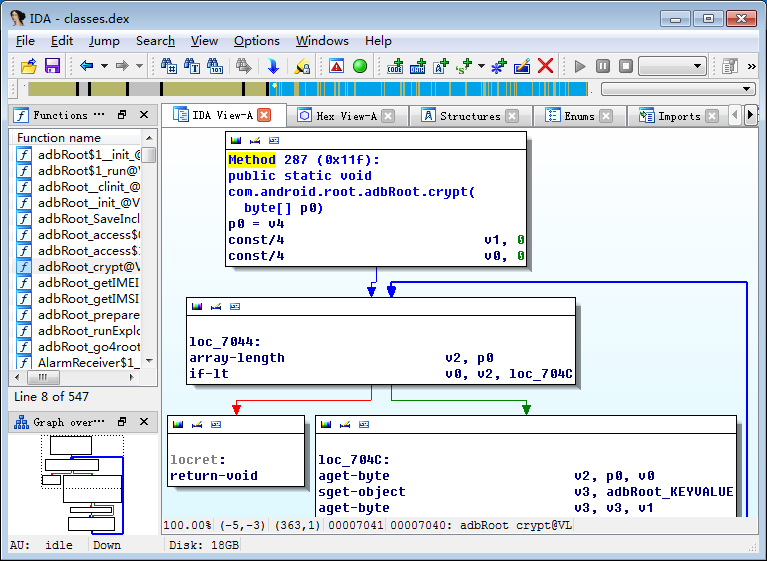
\includegraphics[width=14cm]{image/ida-dex.png}
  \caption{使用IDA Pro反汇编classes.dex文件}
  \label{Fig:ida-dex}
\end{figure}

用IDA Pro分析DEX文件的主要优点是会对函数调用建立交叉索引关系。这在DEX文件被ProGuard混淆后非常有用。因为代码混淆就是通过移除有效的名称信息,降低逆向分析的可理解性,并提高人工查找交叉引用关系和搜索名字的难度。

IDA Pro是一个非常强大的工具,在后面我们还会介绍使用它进行ARM的反汇编和调试。深入学习IDA Pro的使用方法和原理是值得的,而最好的书是\cite{ida_pro}。

\section{Dalvik反编译}
将Java源码编译为Dalvik指令分为两步:先使用\lstinline!javac!将源码编译为.class文件,再使用\lstinline!dx!转换为DEX文件。反之,将DEX文件反编译为Java源码通常也是两步:将DEX再次转换为.class或.jar文件,主要是指令和文件格式的转换;然而将.class或.jar文件用Java反编译器反编译成Java源码。

\subsection{dex2jar}
\lstinline!dex2jar!\footnote{\url{http://code.google.com/p/dex2jar/}}\index{dex2jar}将classes.dex逆向为Java的类文件(.class文件),并打包为.jar格式。

\lstinline!dex2jar!并不直接使用classes.dex,它自带了解析APK的功能,命令为:
\begin{lstlisting}[language=bash, numbers=none]
 $ ./dex2jar Example.apk
\end{lstlisting}
最后在当前目录生成名为Example.apk.dex2jar.jar的文件。

应当注意的是,\lstinline!dex2jar!工具的结果并不完全精确。目前已知在转换\lstinline!switch!、\lstinline!try-exception!等函数结构时,将会出错。

\subsection{jd-gui}
\lstinline!jd-gui!\footnote{\url{http://java.decompiler.free.fr/?q=jdgui}}\index{jd-gui}是一个图形界面的Java反编译器,可以用来反编译\lstinline!dex2jar!产生的jar文件。

\begin{figure}[htbp]
  \centering
  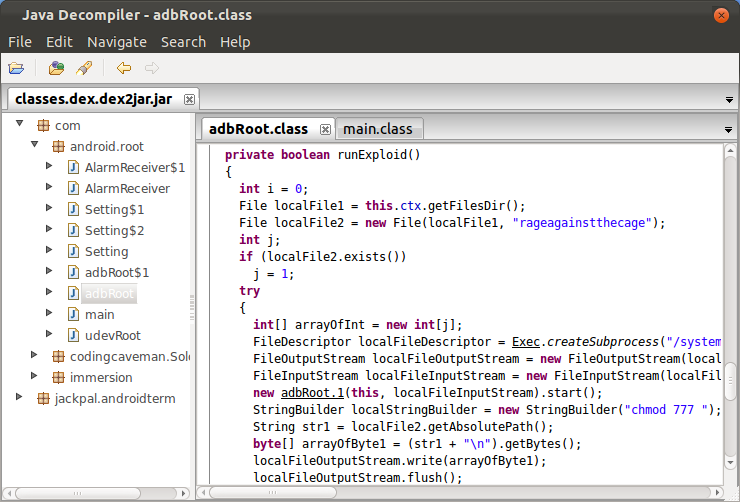
\includegraphics[width=14cm]{image/jd-gui.png}
  \caption{使用jd-gui反编译dex2jar的结果}
  \label{Fig:jd-gui}
\end{figure}

\lstinline!dex2jar!对部分函数结构的逆向错误将直接在\lstinline!jd-gui!的反编译结果中显示出来。此外,部分特殊优化的类方法(函数),\lstinline!jd-gui!的反编译将失败。目前还不清楚原因。

\subsection{ded}
\lstinline!ded!\footnote{\url{http://siis.cse.psu.edu/ded/}}\index{ded}是宾西法尼亚大学研究人员开发的软件,可以将DEX文件转为Java的.class文件。目前只能在Linux和Mac OS X下使用。

\lstinline!ded!使用\lstinline!soot!\footnote{\url{http://www.sable.mcgill.ca/soot/}}\index{soot}对.class文件做优化,优化后反编译得到的Java源文件效果较好,在一些细节上优于\lstinline!dex2jar!和\lstinline!jd-gui!的组合,尤其是对一些循环结构和异常处理代码的反编译上。但soot的运行速度极慢、占用内存较多。

\lstinline!ded!的安装和使用方法请参考其主页的说明。

\subsection{其他}
其他反编译器还有\lstinline!undx!\footnote{\url{http://sourceforge.net/projects/undx/}}\index{undx}和\lstinline!dex-decompiler!\footnote{\url{http://code.google.com/p/dex-decompiler/}}\index{dex-decompiler},但效果如何,还没有试用过。

\lstinline!undx!的作者做过一个介绍其实现原理的报告\cite{dalvik_undx},值得参考。

除了\lstinline!jd-gui!和\lstinline!soot!,常用的Java反编译工具还有\lstinline!jad!\footnote{\url{http://www.varaneckas.com/jad}}\index{jad}和\lstinline!dava!\footnote{\url{http://www.sable.mcgill.ca/dava/}}\index{dava}。

\section{数字签名}
数字签名是Android系统的重要安全机制之一。应用软件要被安装到手机中,必须先签名;要发布到官方市场上,还需要签上为开发者专门颁发的签名。因此,应用软件的数字签名在建立白名单、检测未知恶意代码、判断同源性和家族性等方面有很重要的价值。

可惜的是,Android的签名并不像其他系统那样,而是允许开发者自己为自己颁发签名。所以仅仅从安全的角度看,这一机制只起到了完整性校验的作用。

\subsection{signapk}
\lstinline!signapk!\index{signapk}是Android源码中为APK格式文件签名的程序,其源码位于build/tools/signapk/目录,编译后的结果位于的out/host/linux-x86/framework/目录。用法是:
\begin{lstlisting}[language=bash, numbers=none]
 $ java -jar signapk.jar publickey.x509[.pem] privatekey.pk8 input.apk output.apk
\end{lstlisting}
APK文件经过\lstinline!signapk!签名,再使用\lstinline!zipalign!对齐,就可以安装到手机中了。

\subsection{openssl}
一般情况下,APK文件的签名位于其压缩包的META-INF/CERT.RSA文件中。可以使用\lstinline!openssl!\footnote{\url{http://www.openssl.org}}\index{openssl}工具查看其签名信息:
\begin{lstlisting}[language=bash, numbers=none]
 $ openssl pkcs7 -in CERT.RSA -inform DER -print_certs
\end{lstlisting}

\subsection{keytool}
\lstinline!keytool!\index{keytool}是一个用于生成数字签名和解析数字签名的工具,它是JavaSE的一个组件,在安装JavaSE后即可使用。用它查看APK文件数字签名信息的方法是:
\begin{lstlisting}[language=bash, numbers=none]
 $ keytool -printcert -file META-INF/CERT.RSA
\end{lstlisting}
它的输出结果包括序列号和有效期,比使用\lstinline!openssl!得到的要详细。下面是一个示例:

\begin{lstlisting}[language={}, numbers=none]
Owner: CN=Andorid Debug, OU=Android, O=US, L=Califonie US., ST=Califonie US.
Issuer: CN=Andorid Debug, OU=Android, O=US, L=Califonie US., ST=Califonie US.
Serial number: 4dfdba94
Valid from: Sun Jun 19 17:00:04 CST 2011 until: Tue May 26 17:00:04 CST 2111
Certificate fingerprints:
	 MD5:  CB:00:2E:4C:CD:42:4A:2D:BA:EA:A2:05:FD:F6:63:33
	 SHA1: E2:87:FB:29:33:42:D0:B1:3F:84:10:90:2A:AE:6F:48:77:5C:A6:6D
	 Signature algorithm name: SHA1withRSA
	 Version: 3
\end{lstlisting}

\section{综合工具}
\subsection{apktool}
\lstinline!apktool!\footnote{\url{http://code.google.com/p/android-apktool/}}\index{apktool}是一系列工具的集合。它的功能包括:APK文件解包和打包、AXML编码与解码、资源文件的解包和打包、smali汇编与反汇编、samli调试等。

其中,最常用的功能是解包和打包。解包命令为:
\begin{lstlisting}[language=bash, numbers=none]
 $ ./apktool d Example.apk dir
\end{lstlisting}
会将Example.apk文件解包到dir目录,并自动完成其中AXML文件、资源文件、DEX文件的处理。如果省略dir参数,则解包到APK文件同名目录Example。

打包命令为:
\begin{lstlisting}[language=bash, numbers=none]
 $ apktool b dir New.apk
\end{lstlisting}

而在解包和打包之间,允许对配置文件AndroidManifest.xml、资源文件、smali代码的增加、删除、修改等,而重新打包后得到的APK文件在签名后可以安装到手机中运行。因此,\lstinline!apktool!常被攻击者用于恶意代码植入(参考\ref{Sec:repackage}节)或软件破解。但也可以用于恶意代码分析——增加或修改代码后进行动态分析。

\lstinline!apktool!还提供对smali文件的调试功能,将在\ref{Sec:debug}节进一步介绍。

\subsection{androguard}
\lstinline!androguard!\footnote{\url{http://code.google.com/p/androguard/}}\index{androguard}是一个综合性的Android逆向分析工具,使用Python编写。\lstinline!androguard!的功能非常多,包括:
\begin{itemize}
  \item 1
\end{itemize}

\subsection{apkinspector}

\subsection{dexid}
